\documentclass{article}
\usepackage{graphicx}
\usepackage[margin=1.5cm]{geometry}
\usepackage{amsmath}

\begin{document}

\title{Thursday Reading Assessment: Chapter 3-1 through 3-6}
\author{Prof. Jordan C. Hanson}

\maketitle

\begin{figure}[ht]
\centering
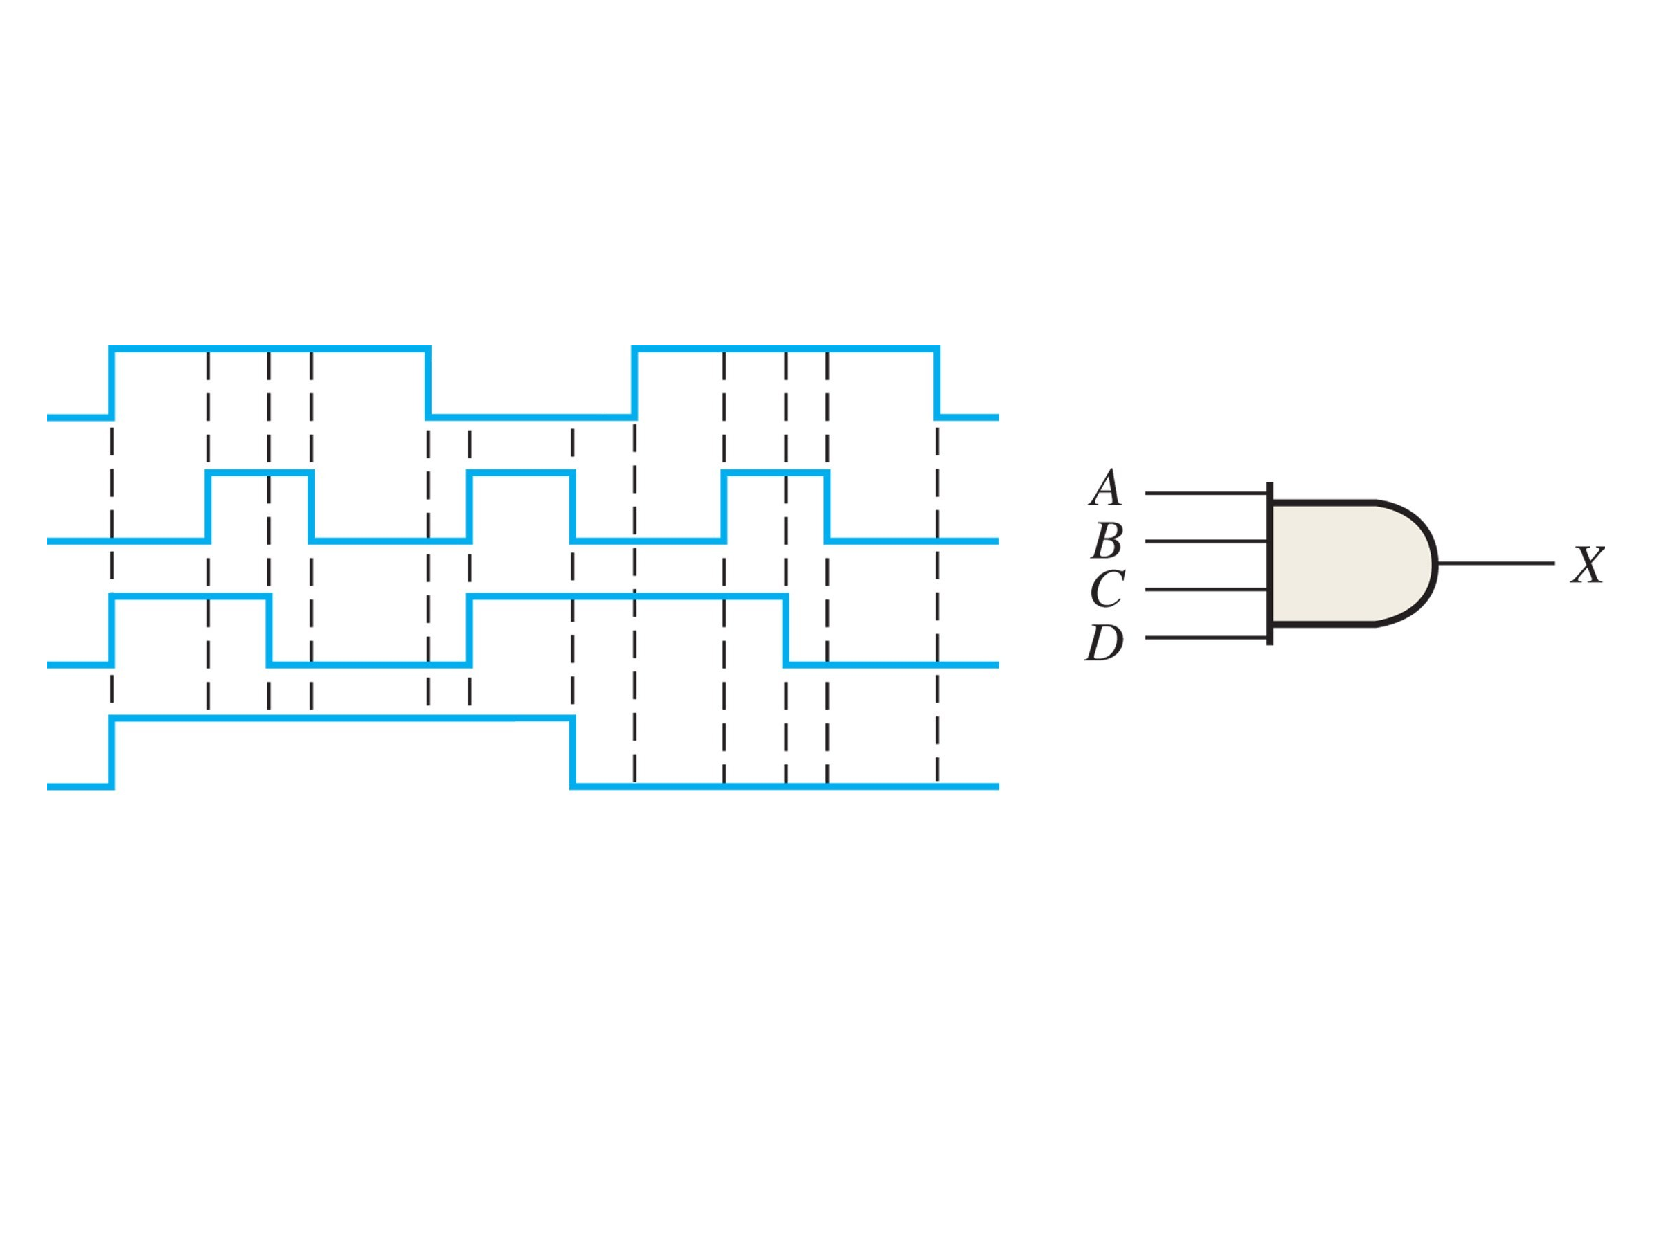
\includegraphics[width=0.45\textwidth,trim=0cm 4cm 0cm 4cm,clip=true]{figures/4and.pdf}
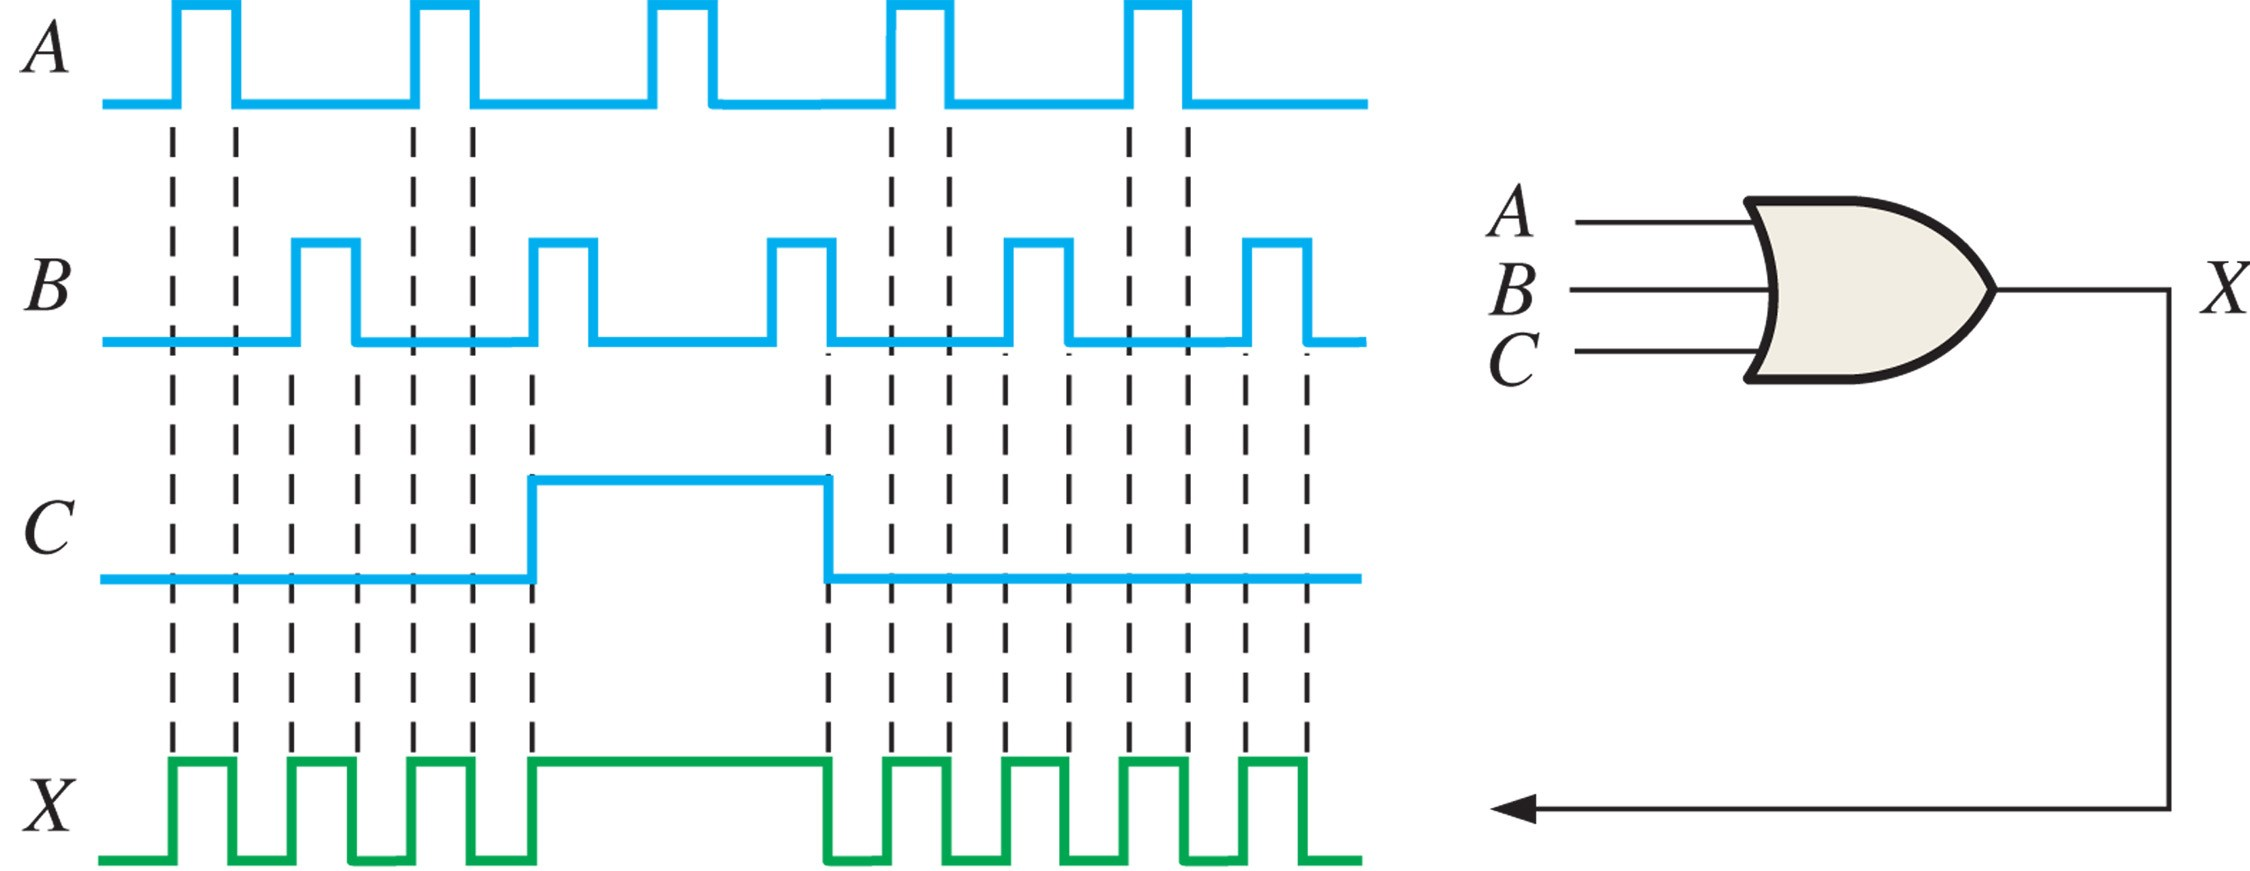
\includegraphics[width=0.45\textwidth,trim=0cm 2cm 0cm 0cm,clip=true]{figures/4OR.jpg}
\caption{\label{fig:4and} (Left) A timing diagram as input to a 4-input AND gate. (Right) A timing diagram as input to a 3-input OR gate.}
\end{figure}

\section{Logic Gates: AND, OR, NOT}

\begin{enumerate}
\item Draw the output timing diagram for the 4-input AND gate in Fig. \ref{fig:4and} (left). \\ \vspace{0.5cm}
\item (a) Draw the output timing diagram for the 3-input OR gate in Fig. \ref{fig:4and} (right). (b) Add the inverted output to your diagram, as if the output was split off into a NOT gate. \\ \vspace{0.5cm}
\end{enumerate}

\section{Logic Gates: NAND, OR, NOT}

\begin{enumerate}
\item (a) If both Tank A and B levels in Fig. \ref{fig:tanks} (left) are below the level sensors, will the green LED be on or off? (b) If both Tank A and B levels in Fig. \ref{fig:tanks} (right) are above the level sensors, will the red LED be on or off? (c) Write the truth table for the gates in Fig. \ref{fig:tanks} (left and right).
\end{enumerate}

\begin{figure}[hb]
\centering
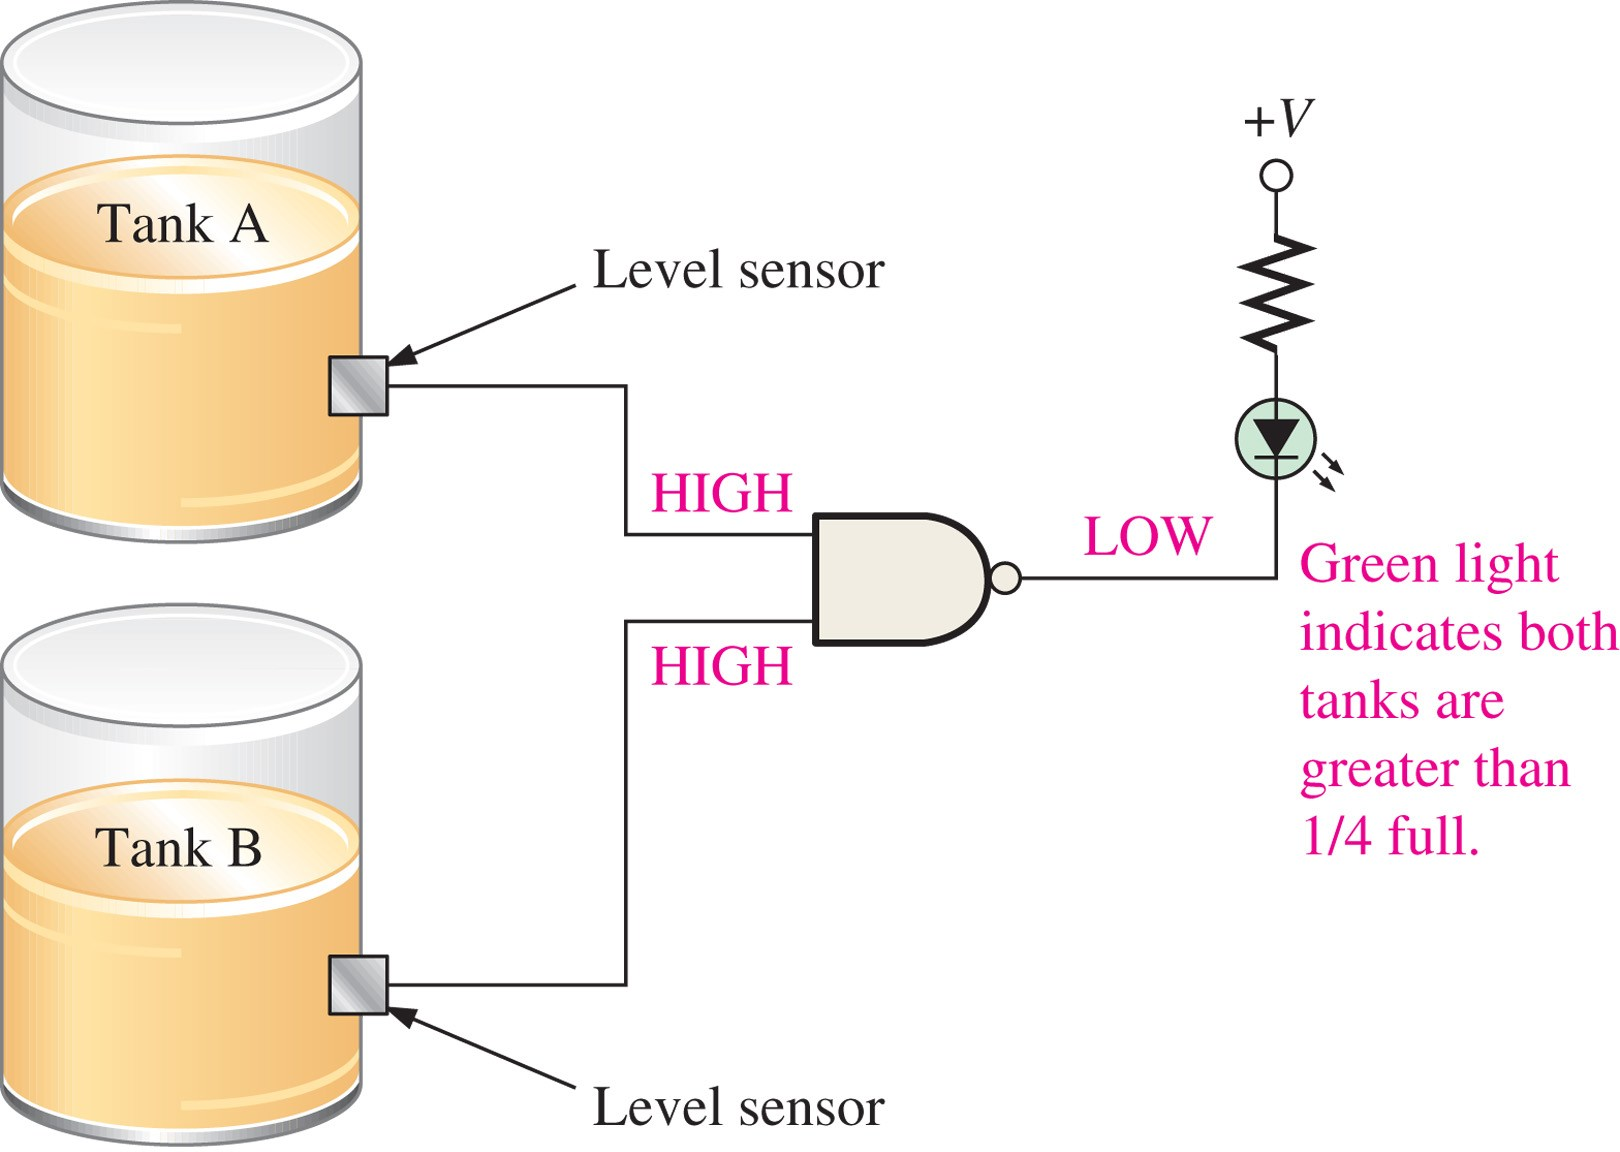
\includegraphics[width=0.3\textwidth]{figures/tank_nand_1.jpg} \hspace{0.5cm}
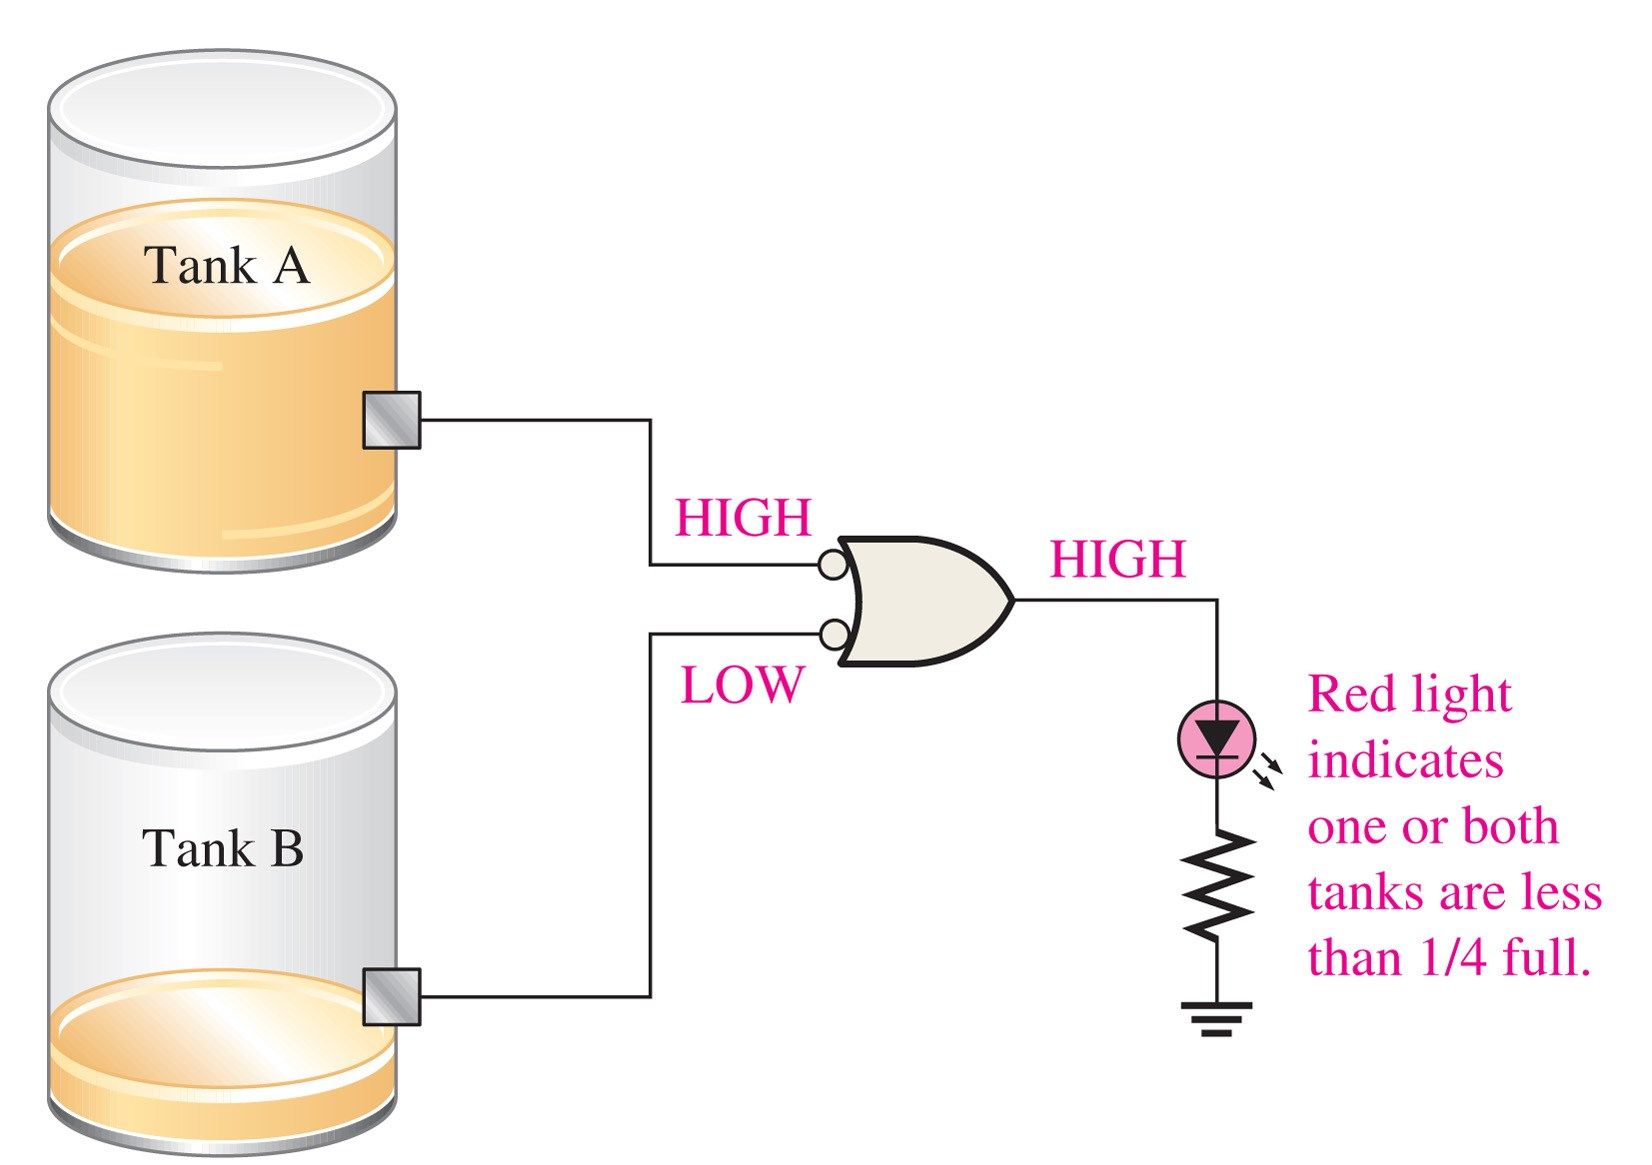
\includegraphics[width=0.3\textwidth]{figures/tank_nand_2.jpg}
\caption{\label{fig:tanks} (Left) A timing diagram as input to a 4-input AND gate. (Right) A timing diagram as input to a 3-input OR gate.}
\end{figure}


\end{document}
